\documentclass[12pt,fleqn]{article}\usepackage{../common}
\begin{document}
Coklu Bakis Noktali Geometri (Multiple View Geometry)

[1, sf. 145]

\begin{minted}[fontsize=\footnotesize]{python}
import pandas as pd
import siftpy1
df1 = siftpy1.sift('alcatraz1s.pgm', threshold=10.0)
df2 = siftpy1.sift('alcatraz2s.pgm', threshold=10.0)
\end{minted}

\begin{minted}[fontsize=\footnotesize]{python}
from PIL import Image
im1=Image.open("alcatraz1s.jpg")
im2=Image.open("alcatraz2s.jpg")
df1.plot(kind='scatter',x=0,y=1)
plt.hold(True)
plt.imshow(im1)
plt.savefig('mvg_01.png')
\end{minted}

\begin{minted}[fontsize=\footnotesize]{python}
df2.plot(kind='scatter',x=0,y=1)
plt.hold(True)
plt.imshow(im2)
plt.savefig('mvg_02.png')
\end{minted}


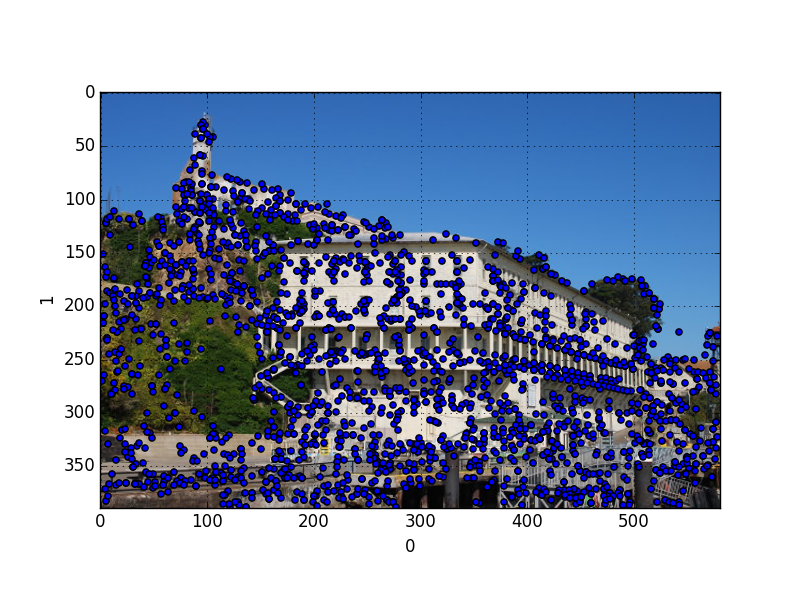
\includegraphics[height=6cm]{mvg_01.png}
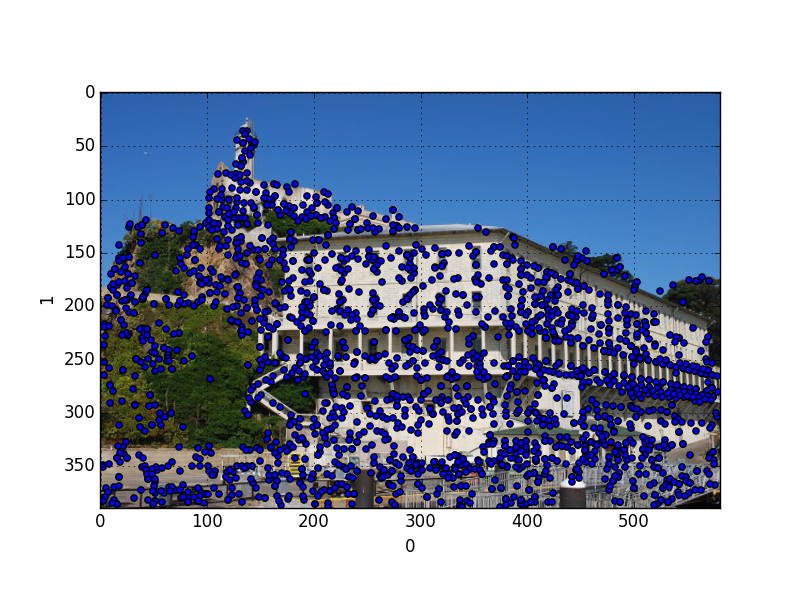
\includegraphics[height=6cm]{mvg_02.png}

\begin{minted}[fontsize=\footnotesize]{python}
matches = siftpy1.match_twosided(df1,df2)
\end{minted}

\begin{minted}[fontsize=\footnotesize]{python}
print matches[:10]
\end{minted}

\begin{verbatim}
[  0 662   1   3   0   0   0   0   0  10]
\end{verbatim}

\begin{minted}[fontsize=\footnotesize]{python}
import homography
import sfm
# calibration
K = np.array([[2394,0,932],[0,2398,628],[0,0,1]])
\end{minted}


\begin{minted}[fontsize=\footnotesize]{python}
import numpy.linalg as lin
l1 = np.array(df1)[:,:4]
l2 = np.array(df2)[:,:4]

ndx = matches.nonzero()[0]
# make homogeneous and normalize with lin.inv(K)
x1 = homography.make_homog(l1[ndx,:2].T)
ndx2 = [int(matches[i]) for i in ndx]
x2 = homography.make_homog(l2[ndx2,:2].T)
x1n = np.dot(lin.inv(K),x1)
x2n = np.dot(lin.inv(K),x2)

# estimate E with RANSAC
model = sfm.RansacModel()
E,inliers = sfm.F_from_ransac(x1n,x2n,model)
\end{minted}

\begin{minted}[fontsize=\footnotesize]{python}
# compute camera matrices (P2 will be list of four solutions)
P1 = np.array([[1,0,0,0],[0,1,0,0],[0,0,1,0]])
P2 = sfm.compute_P_from_essential(E)

# pick the solution with points in front of cameras
ind = 0
maxres = 0
for i in range(4):
    # triangulate inliers and compute depth for each camera
    X = sfm.triangulate(x1n[:,inliers],x2n[:,inliers],P1,P2[i])
    d1 = np.dot(P1,X)[2]
    d2 = np.dot(P2[i],X)[2]
    if np.sum(d1>0)+np.sum(d2>0) > maxres:
        maxres = np.sum(d1>0)+np.sum(d2>0)
        ind = i
        infront = (d1>0) & (d2>0)

# triangulate inliers and remove points not in front of both cameras
X = sfm.triangulate(x1n[:,inliers],x2n[:,inliers],P1,P2[ind])
X = X[:,infront]
\end{minted}


\begin{minted}[fontsize=\footnotesize]{python}
# 3D plot
from mpl_toolkits.mplot3d import axes3d
fig = plt.figure()
ax = fig.gca(projection='3d')
ax.plot(-X[0],X[1],X[2],'k.')
plt.axis('off')
plt.savefig('mvg_03.png')
\end{minted}

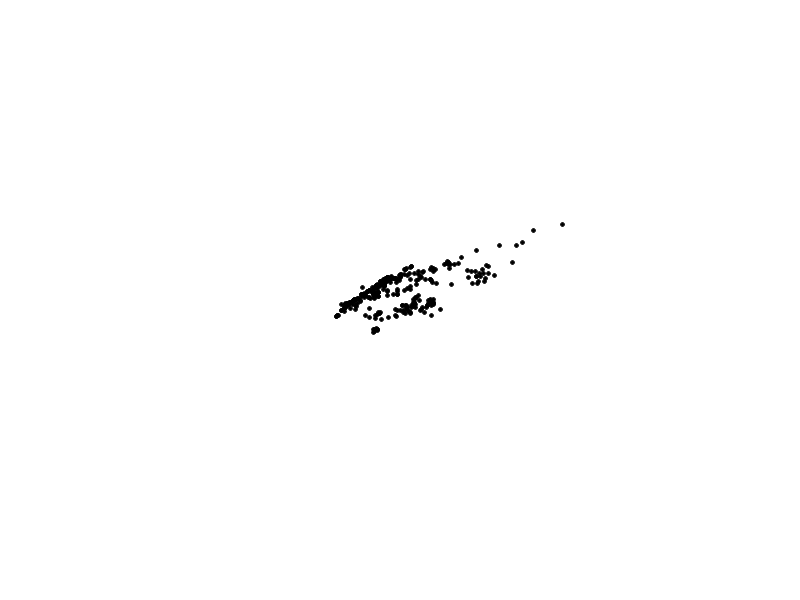
\includegraphics[height=6cm]{mvg_03.png}


\begin{minted}[fontsize=\footnotesize]{python}
w = 620; h = 465
from PIL import Image
im = Image.open('out-cam.png')
plt.imshow(im)
x = [[228, 398],[249, 338],[123, 245],\
     [121, 186],[278, 248],[488,205],\
     [291,194],[432,167],[73,288],[123,130]]
X = [[20,0,21],[20,0,22],[18,0,30],\
     [18,1,30],[20,0,30],[22,2,21],\
     [20,1,30],[22,2,22],[18,0,25],[18,2,30]]
for i in range(len(x)): 
    plt.plot(x[i][0],x[i][1],'r+')
    plt.text(x[i][0]+2,x[i][1]+2,str(X[i]),color='cyan')
plt.savefig('out-cam2.png')
\end{minted}


\begin{minted}[fontsize=\footnotesize]{python}
xx = np.array(x)
xx[:,1] = h-xx[:,1]
xx = np.hstack((xx,np.ones((len(x),1))))
print xx

XX = np.array(X)
XX = np.hstack((XX,np.ones((len(X),1))))
print XX
\end{minted}

\begin{verbatim}
[[ 228.   67.    1.]
 [ 249.  127.    1.]
 [ 123.  220.    1.]
 [ 121.  279.    1.]
 [ 278.  217.    1.]
 [ 488.  260.    1.]
 [ 291.  271.    1.]
 [ 432.  298.    1.]
 [  73.  177.    1.]
 [ 123.  335.    1.]]
[[ 20.   0.  21.   1.]
 [ 20.   0.  22.   1.]
 [ 18.   0.  30.   1.]
 [ 18.   1.  30.   1.]
 [ 20.   0.  30.   1.]
 [ 22.   2.  21.   1.]
 [ 20.   1.  30.   1.]
 [ 22.   2.  22.   1.]
 [ 18.   0.  25.   1.]
 [ 18.   2.  30.   1.]]
\end{verbatim}


\begin{minted}[fontsize=\footnotesize]{python}
import sfm
P = sfm.compute_P(xx.T,XX.T)
print P
\end{minted}

\begin{verbatim}
[[ -3.51453236e-02   6.07296303e-03  -4.77554122e-03   7.60267630e-01]
 [ -2.60992369e-02   2.86474695e-03  -6.65011035e-03   6.48041916e-01]
 [ -1.05982107e-04   5.38385833e-05  -2.14097132e-05   2.43755206e-03]]
\end{verbatim}

\begin{minted}[fontsize=\footnotesize]{python}
w = 620; h = 465
from PIL import Image
im = Image.open('out-cam.png')
plt.imshow(im)
X2 = np.dot(P, np.array([[20,0,22,1]]).T ) 
X2 = X2 / X2[2]
print X2
plt.plot(X2[0],h-X2[1],'d')
plt.savefig('out-cam3.png')
\end{minted}

\begin{verbatim}
[[ 311.55831094]
 [ 132.23221819]
 [   1.        ]]
\end{verbatim}

\begin{minted}[fontsize=\footnotesize]{python}
res1 = np.array([[18, 0, 20+i, 1.] for i in np.linspace(0,30,100)])
res2 = np.array([[21, 0, 20+i, 1.] for i in np.linspace(0,30,100)])

X3 = np.dot(P, res1.T)
X3 = X3 / X3[2]
im = Image.open('out-cam.png')
plt.imshow(im)

for xx in X3.T: 
    plt.hold(True)
    if xx[0] > w or xx[0] < 0: continue
    if xx[1] > h or xx[1] < 0: continue
    plt.plot(xx[0],h-xx[1],'r.')

plt.hold(True)

X3 = np.dot(P, res2.T)
X3 = X3 / X3[2]
for xx in X3.T: 
    plt.hold(True)
    if xx[0] > w or xx[0] < 0: continue
    if xx[1] > h or xx[1] < 0: continue
    plt.plot(xx[0],h-xx[1],'r.')

plt.savefig('out-cam4.png')
\end{minted}















Kaynaklar

[1] Solem, {\em Computer Vision with Python}

\end{document}
